\documentclass{../../../oss-ap12ibhl}
\usepackage{multicol}

\begin{document}
\genheader

\gentitle{2}{DYNAMICS}

\begin{questions}
  \question A small moving block collides with a large block at rest. Which of
  the following is true of the forces the blocks apply to each other
  \begin{choices}
    \choice The small block exerts twice the force on the large block
    compared to the force the large block exerts on the small block.
    \choice The small block exerts half the force on the large block compared
    to the force the large block exerts on the small block.
    \choice The small block exerts exactly the same amount of force on the
    large block that the large block exerts on the small block.
    \choice The large block exerts a force on the small block, but the small
    block does not exert a force on the large block.
    \choice The small block exerts a force on the large block, but the large
    block does not exert a force on the small block.
  \end{choices}
  \vspace{.7in}
  
%  \item Which of the following position vs. time graphs shows an example of
%    the law of inertia?
%    \pic{.2}{law-of-inertia.png}

%  \uplevel{
%    \textbf{Questions \ref{q:2blocks1}-\ref{q:2blocks2}}
%
%    Two blocks, \SI{4.}{\kilo\gram} and \SI{2.}{\kilo\gram}, are connected by a
%    string. An applied force $F$ of magnitude \SI{18}{\newton} pulls the blocks
%    to the left.
%    \cpic{.38}{connect1}
%  }
%  
%  \question The acceleration of the \SI{4.}{\kilo\gram} block is
%  \begin{choices}
%    \choice\SI{2.0}{\metre\per\second\squared}
%    \choice\SI{3.0}{\metre\per\second\squared}
%    \choice\SI{4.0}{\metre\per\second\squared}
%    \choice\SI{4.5}{\metre\per\second\squared}
%    \choice\SI{6.0}{\metre\per\second\squared}
%  \end{choices}
%  \label{q:2blocks1}
%  
%  \question The tension in the string between the blocks is
%  \begin{choices}
%    \choice 4.0 N
%    \choice 6.0 N
%    \choice 12 N
%    \choice 16 N
%    \choice 18 N
%  \end{choices}
%  \label{q:2blocks2}

  \uplevel{
    \textbf{Questions \ref{q:pulley1}--\ref{q:pulley2}}

    A system consists of two blocks having masses of \SI{2}{\kilo\gram} and
    \SI{1}{\kilo\gram}. The blocks are connected by a string of negligible mass
    and hung over a light pulley, and then released from rest.
    \begin{center}
      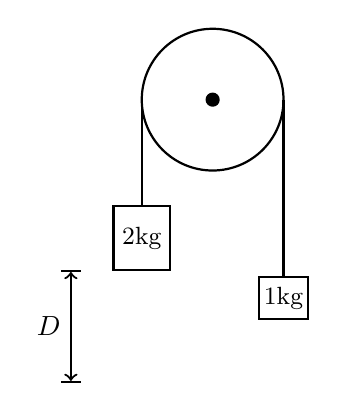
\begin{tikzpicture}[scale=.9]
        \draw[thick](0,0) circle(1);
        \fill(0,0) circle(.1);
        \draw[thick](-1,0)--(-1,-1.5);
        \draw[thick](-1.4,-1.5)rectangle(-.6,-2.4)
        node[midway]{\small\SI{2}{kg}};
        \draw[thick](1,0)--(1,-2.5);
        \draw[thick](.65,-2.5)rectangle(1.35,-3.1)
        node[midway]{\small\SI{1}{kg}};
        \draw[thick,|<->|](-2,-2.4)--(-2,-4) node[midway,left]{$D$};
      \end{tikzpicture}
    \end{center}
  }

  \question The acceleration of the \SI{2}{\kilo\gram} block is most nearly
  \begin{choices}
    \choice $\dfrac29g$
    \choice $\dfrac13g$
    \choice $\dfrac12g$
    \choice $\dfrac23g$
    \choice $g$
  \end{choices}
  \label{q:pulley1}
    
  \question The speed of the \SI{2}{\kilo\gram} block after it has descended a
  distance $D$ is most nearly
  \begin{choices}
    \choice $\sqrt{\dfrac{4gD}{3}}$
    \choice $\sqrt{\dfrac{2gD}{3}}$
    \choice $\sqrt{\dfrac{gD}{3}}$
    \choice $\sqrt{\dfrac{gD}{2}}$
    \choice $\sqrt{\dfrac{4gD}{6}}$
  \end{choices}
  \label{q:pulley2}

%  \uplevel{
%    \textbf{Questions \ref{q:2cords1}--\ref{q:2cords2}}
%
%    A weight of magnitude $W$ is suspended in equilibrium by two cords, one
%    horizontal and one slanted at an angle of \ang{60} from the horizontal, as
%    shown.
%    \cpic{.33}{hang1}
%  }
%  
%  \question Which of the following statements is true?
%  \begin{choices}
%    \choice The tension in the horizontal cord must be greater than the tension
%      in the slanted cord.
%    \choice The tension in the slanted cord must be greater than the tension in
%      the horizontal cord.
%    \choice The tension is the same in both cords.
%    \choice The tension in the horizontal cord equals the weight $W$.
%    \choice The tension in the slanted cord equals the weight $W$.
%  \end{choices}
%  \label{q:2cords1}
%    
%  \question The tension in the horizontal cord is
%  \begin{choices}
%    \choice equal to the tension in the slanted cord
%    \choice one-third as much as the tension in the slanted cord
%    \choice one-half as much as the tension in the slanted cord
%    \choice twice as much as the tension in the slanted cord
%    \choice three times as much as the tension in the slanted cord
%  \end{choices}
%  \label{q:2cords2}
  
  \question A wooden block slides down a frictionless inclined plane a distance
  of 1 meter along the plane during the first second. The distance traveled
  along the plane by the block during the time between \SI{1}{s} and \SI{2}{s}
  is
  \begin{choices}
    \choice\SI{2}{\metre}
    \choice\SI{3}{\metre}
    \choice\SI{4}{\metre}
    \choice\SI{6}{\metre}
    \choice\SI{8}{\metre}
  \end{choices}

%  \question A weight $W$ is hung from two threads, $A$ and $B$, as shown below.
%  The magnitudes of the tensions in each string are $F_A$ and $F_B$,
%  respectively. Which of the following describes the relationship between
%  $F_A$, $F_B$, and $W$?
%  \cpic{.25}{hang-weight.png}
%  \begin{choices}
%    \choice $F_A=F_B=W$
%    \choice $F_A=F_B$
%    \choice $F_A<F_B$
%    \choice $F_A>F_B$
%    \choice $F_A+F_B=W$
%  \end{choices}
  
  \uplevel{
    \textbf{Questions \ref{3blks1}--\ref{3blks2}}

    Three blocks of mass \SI{3}{\kilo\gram}, \SI{2}{\kilo\gram}, and
    \SI{1}{\kilo\gram} are pushed along a horizontal frictionless plane by a
    force of \SI{24}{\newton} to the right, as shown.
    \begin{center}
      \begin{tikzpicture}[scale=.75]
        \fill[pattern=north east lines] (0,0) rectangle(8,-.3);
        \begin{scope}[thick]
          \draw (0,0)--(8,0);
          \draw (2,0) rectangle(4,1.5) node[midway]{3 kg};
            \draw (4,0) rectangle(5.5,1.3) node[midway]{2 kg};
            \draw (5.5,0) rectangle(6.5,1.1) node[midway]{1 kg};
            \draw[->](0,.75)--(2,.75) node[midway,above]{24 N};
        \end{scope}
      \end{tikzpicture}
    \end{center}
  }

  \question The acceleration of the \SI{2}{\kilo\gram} block is
  \begin{choices}
    \choice\SI{144}{\metre\per\second\squared}
    \choice\SI{72}{\metre\per\second\squared}
    \choice\SI{12}{\metre\per\second\squared}
    \choice\SI{6}{\metre\per\second\squared}
    \choice\SI{4}{\metre\per\second\squared}
  \end{choices}
  \label{3blks1}
    
  \question The force that the \SI{2}{\kilo\gram} block exerts on the
  \SI{1}{\kilo\gram} block is
  \begin{choices}
    \choice\SI{2}{\newton}
    \choice\SI{4}{\newton}
    \choice\SI{6}{\newton}
    \choice\SI{24}{\newton}
    \choice\SI{144}{\newton}
  \end{choices}
  \label{3blks2}
    
  \question A hockey puck slides along horizontal ice with a velocity $\bm{v}_1$
  when it is struck by a hockey stick, changing its direction, as shown. After
  the puck is struck, it has a velocity $\bm{v}_2$, which is greater than
  $\bm{v}_1$. Which of the following vectors best represents the direction the
  force of the hockey stick acted on the puck?
  \begin{center}
    \begin{tikzpicture}[scale=.6]
      \draw[ultra thick,->](0,0)--(2,0) node[midway,below]{$\bm{v}_1$};
      \draw[ultra thick,->](4,0)--(4,2.5) node[midway,right]{$\bm{v}_2$};
      \draw[dashed](0,0)--(4,0)--(4,3.5);
    \end{tikzpicture}
  \end{center}
  \begin{oneparchoices}
    \choice{\Huge $\uparrow$}
    \choice{\Huge $\leftarrow$}
    \choice{\Huge $\rightarrow$}
    \choice{\Huge $\nwarrow$}
    \choice{\Huge $\nearrow$}
  \end{oneparchoices}
  \vspace{.2in}
  
  \question A block of mass \SI{4}{\kilo\gram} slides down a rough incline with
  a constant speed. The angle the incline makes with the horizontal is
  \ang{30}. The coefficient of friction acting between the block and incline
  is most nearly

  \begin{minipage}{.3\linewidth}
    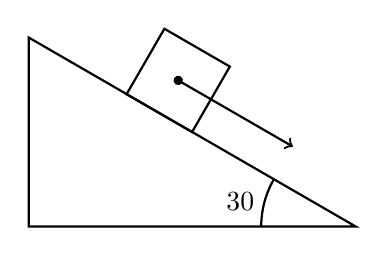
\begin{tikzpicture}[scale=1.2]
      \begin{scope}[thick]
        \draw(0,0)--(-3.46,0)--(-3.46,2)--cycle;
        \draw[thick](-1,0) arc(180:150:1) node[midway,left]{\ang{30}};
        \begin{scope}[rotate=-30]
          \draw(-2,0) rectangle(-2.8,.8);
          \fill(-2.4,.4) circle(.05);
          \draw[->](-2.4,.4)--(-1.,.4)node[right]{$\varv$};
        \end{scope}
      \end{scope}
    \end{tikzpicture}
  \end{minipage}
  \begin{minipage}{.4\linewidth}
    \begin{choices}
      \choice 0.1
      \choice 0.2
      \choice 0.3
      \choice 0.4
      \choice 0.6
    \end{choices}
  \end{minipage}
    
%  \question A ball is thrown straight up into the air, encountering air
%  resistance as it rises. What forces, if any, act on the ball as it rises?
%  \begin{choices}
%    \choice A decreasing gravitational force and an increasing force of air
%    resistance
%    \choice An increasing gravitational force and an increasing force of air
%    resistance
%    \choice A decreasing gravitational force and a decreasing force of air
%    resistance
%    \choice A constant gravitational force and an increasing force of air
%    resistance
%    \choice A constant gravitational force and a decreasing force of air
%    resistance
%  \end{choices}

  \question Two blocks are pulled by a force of magnitude $F$ along a level
  surface with negligible friction as shown. The tension in the string between
  the blocks is
  \cpic{.35}{connect2}
  \begin{choices}
    \choice $\dfrac14F$
    \choice $\dfrac12F$
    \choice $\dfrac13F$
    \choice $F$
    \choice $2F$
  \end{choices}
  
  \question A block of mass $4m$ can move without friction on a horizontal
  surface. Another block of mass $m$ is attached to the larger block by a
  string that is passed over a light pulley. The acceleration of the system is
  \cpic{.3}{atwood1}
  \begin{choices}
    \choice $\dfrac15g$
    \choice $\dfrac12g$
    \choice $\dfrac23g$
    \choice $g$
    \choice $5g$
  \end{choices}

  \question The block of mass $4m$ in the previous question now moves on a rough
  surface. The frictional force between the surface and the larger block is
  equal to $\dfrac12mg$. The acceleration of the system is now
  \begin{choices}
    \choice $\dfrac1{16}g$
    \choice $\dfrac1{10}g$
    \choice $\dfrac1{4}g$
    \choice $\dfrac1{2}g$
    \choice $g$
  \end{choices}
    
%  \question A force of magnitude $F$ pulls up at an angle $\theta$ to the
%  horizontal on a block of mass $m$. The mass remains in contact with the
%  level floor and the coefficient of friction between the block and the floor
%  is $\mu$. The frictional force between the floor and the block is
%  \begin{center}
%    \pic{.2}{angle1.png}
%  \end{center}
%  \begin{choices}
%    \choice$\mu mg$
%    \choice$\mu (mg-F\sin\theta)$
%    \choice$\mu (mg+F\sin\theta)$
%    \choice$\mu (mg-F\cos\theta)$
%    \choice$\mu (mg+F\cos\theta)$
%  \end{choices}
  \newpage
  
  \uplevel{
    \textbf{Questions \ref{fbds}--\ref{fk}}

    A \SI{1}{\kilo\gram} block is sliding up a rough \ang{30} incline and is
    slowing down with an acceleration of \SI{-6}{\metre\per\second\squared}. The
    mass has a weight $\bm{w}$, and encounters a frictional force $\bm{f}$ and a
    normal force $\bm{N}$. The direction up the ramp is positive.
    \cpic{.25}{ramp2}
  }

  \question Which of the following free body diagrams best represents the forces
  acting on the block as it slides up the plane?
  \begin{oneparchoices}
    \choice
    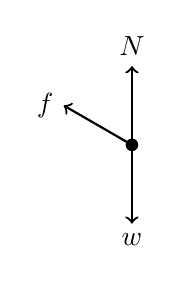
\begin{tikzpicture}
      \fill[black](0,0) circle(.08);
      \draw[thick,->](0,0)--(0,1)node[above]{$\bm{N}$};
      \draw[thick,->](0,0)--(0,-1)node[below]{$\bm{w}$};
      \draw[thick,->,rotate=60](0,0)--(0,1)node[left]{$\bm{f}$};
    \end{tikzpicture}
    \choice
    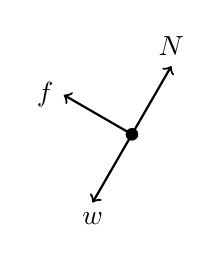
\begin{tikzpicture}
      \fill[black](0,0) circle(.08);
      \draw[thick,->,rotate=-30](0,0)--(0,1)node[above]{$\bm{N}$};
      \draw[thick,->,rotate=-30](0,0)--(0,-1)node[below]{$\bm{w}$};
      \draw[thick,->,rotate=60](0,0)--(0,1)node[left]{$\bm{f}$};
    \end{tikzpicture}
    \choice
    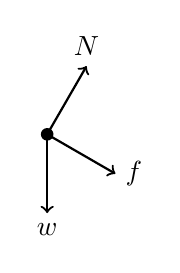
\begin{tikzpicture}
      \fill[black](0,0) circle(.08);
      \draw[thick,->,rotate=-30](0,0)--(0,1)node[above]{$\bm{N}$};
      \draw[thick,->](0,0)--(0,-1)node[below]{$\bm{w}$};
      \draw[thick,->,rotate=60](0,0)--(0,-1)node[right]{$\bm{f}$};
    \end{tikzpicture}
    \choice
    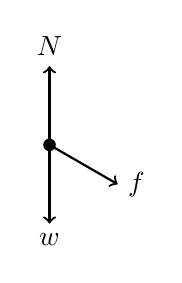
\begin{tikzpicture}
      \fill[black](0,0) circle(.08);
      \draw[thick,->](0,0)--(0,1)node[above]{$\bm{N}$};
      \draw[thick,->](0,0)--(0,-1)node[below]{$\bm{w}$};
      \draw[thick,->,rotate=60](0,0)--(0,-1)node[right]{$\bm{f}$};
    \end{tikzpicture}
    \choice
    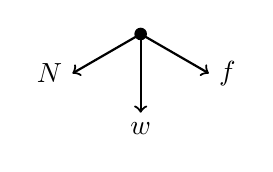
\begin{tikzpicture}
      \fill[black](0,0) circle(.08);
      \draw[thick,->,rotate=120](0,0)--(0,1)node[left]{$\bm{N}$};
      \draw[thick,->](0,0)--(0,-1)node[below]{$\bm{w}$};
      \draw[thick,->,rotate=60](0,0)--(0,-1)node[right]{$\bm{f}$};
    \end{tikzpicture}
    \end{oneparchoices}
    \label{fbds}
    
  \question The magnitude of the frictional force $f$ between the block and the
  plane is most nearly
  \begin{choices}
    \choice\SI{1}{\newton}
    \choice\SI{2}{\newton}
    \choice\SI{3}{\newton}
    \choice\SI{4}{\newton}
    \choice\SI{5}{\newton}
  \end{choices}
  \label{fk}

%  \item A block weighing \SI{60}{\newton} hangs from three ropes as shown.
%    Which of the following statements is true?
%    \begin{center}
%      \vspace{-.1in}\pic{.3}{hanging.png}
%    \end{center}
%    \begin{choices}    
%    \choice Each rope has a tension of \SI{60}{\newton}.
%    \choice The tension in each rope is higher in the lower part than in the
%      upper part of the rope.
%    \choice The tension in each rope is higher in the upper part than in the
%      lower part of the rope.
%    \choice The rope in the center has a higher tension than the othertwo ropes.
%    \choice Each rope has a tension of \SI{20}{\newton}.
%    \end{choices}
  
  \question Three strings are attached to a ring in the center of a force
  table. The top view of the force table is shown. For the ring to remain in the
  center of the table, which of the following must be true?

  \begin{minipage}{.3\linewidth}
    \centering
    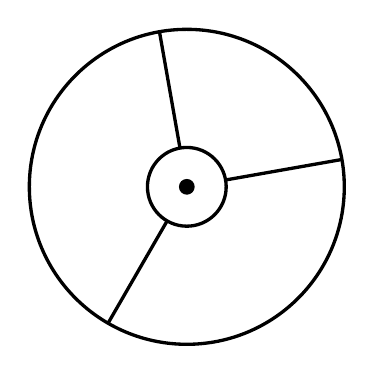
\begin{tikzpicture}[scale=2]
      \draw[very thick](0,0) circle(1);
      \draw[very thick](0,0) circle(.25);
      \fill            (0,0) circle(.05);
      \draw[very thick,rotate=10] (.25,0)--(1,0);
      \draw[very thick,rotate=100](.25,0)--(1,0);
      \draw[very thick,rotate=240](.25,0)--(1,0);
    \end{tikzpicture}
  \end{minipage}
  \begin{minipage}{.68\linewidth}
    \begin{choices}
      \choice The vector sum of the three forces must equal zero.
      \choice The lengths of the strings must be equal.
      \choice The strings must form an angle of \ang{90} relative to each other.
      \choice The magnitudes of two of the tensions in the strings must equal
      the tension in the third string.
      \choice The tension in each string must be equal to each other.
    \end{choices}
  \end{minipage}
  \vspace{.2in}
  
  \uplevel{
    \textbf{Questions \ref{plane1}--\ref{plane2}}

    A \SI{10}{\newton} block sits atop an inclined plane in the shape of a
    right triangle of sides \SI{3}{\metre}, \SI{4}{\metre}, and \SI{5}{\metre},
    as shown. The block is allowed to slide down the plane with negligible
    friction.
    \begin{center}
      \begin{tikzpicture}
        \draw(0,0) --(0,-3)node[midway,left]{3 m};
        \draw(0,-3)--(4,-3)node[midway,below]{4 m};
        \draw(4,-3)--(0,0)node[midway,above right]{5 m};
        \draw[rotate=-atan(3/4)](0,0) rectangle(.8,.8) node[above right]{10 N};
      \end{tikzpicture}
    \end{center}
  }

  \question The acceleration of the block is most nearly
  \begin{choices}
    \choice\SI{2}{\metre\per\second\squared}
    \choice\SI{4}{\metre\per\second\squared}
    \choice\SI{6}{\metre\per\second\squared}
    \choice\SI{10}{\metre\per\second\squared}
    \choice\SI{12}{\metre\per\second\squared}
  \end{choices}
  \label{plane1}
    
  \question The normal force exerted on the block by the plane is most nearly
  \begin{choices}
    \choice\SI{2}{\newton}
    \choice\SI{4}{\newton}
    \choice\SI{6}{\newton}
    \choice\SI{8}{\newton}
    \choice\SI{10}{\newton}
  \end{choices}
  \label{plane2}
  
  \question A constant force acts on a particle in such a way that the
  direction of the force is always perpendicular to its velocity. Which of the
  following is true of the particle's motion?
  \begin{choices}
    \choice The acceleration of the particle is increasing
    \choice The acceleration of the particle is decreasing.
    \choice The speed of the particle is increasing.
    \choice The speed of the particle is constant.
    \choice The speed of the particle is decreasing.
  \end{choices}

  \uplevel{
    \textbf{Questions \ref{stacked1}--\ref{stacked2}}

    A block of mass \SI{2}{\kilo\gram} rests on top of a larger block of mass
    \SI{4}{\kilo\gram}. The larger block slides without friction on a table, but
    the surface between the two blocks is not frictionless. The coefficient of
    friction between the two blocks is 0.2. A horizontal force $\bm{F}$ is
    applied to the \SI{4}{\kilo\gram} mass.
    \cpic{.4}{stacked}
  }

  \question What is the maximum force that can be applied such that there is no
  relative motion between the two blocks?
  \begin{choices}
    \choice zero
    \choice\SI{1}{\newton}
    \choice\SI{2}{\newton}
    \choice\SI{4}{\newton}
    \choice\SI{12}{\newton}
  \end{choices}
  \label{stacked1}
  
  \question What is the acceleration of the \SI{2}{\kilo\gram} block relative
  to the \SI{4}{\kilo\gram} block if a force is applied to the
  \SI{4}{\kilo\gram} block that causes the \SI{4}{\kilo\gram} block to
  accelerate at \SI{3}{\metre\per\second\squared} to the right?
  \begin{choices}
    \choice\SI{1}{\metre\per\second\squared} to the right
    \choice\SI{1}{\metre\per\second\squared} to the left
    \choice\SI{2}{\metre\per\second\squared} to the right
    \choice\SI{2}{\metre\per\second\squared} to the left
    \choice zero
  \end{choices}
  \label{stacked2}
  \newpage

%\item Two balls are thrown with equal speeds $v_0$ from the top of a cliff of
%  height $H$. One ball is thrown upward at an angle $\alpha$ above the
%  horizontal; the other ball is thrown downward at an angle of $\beta$ below
%  the horizontal. Show that each ball strikes the ground with the same speed,
%  and find that speed in terms of $H$ and the initial speed $v_0$.
%  \vspace{2in}
%  \newpage

  % THIS QUESTION IS FROM THE 2000 AP PHYSICS B EXAM, QUESTION 2
  \uplevel{
    \cpic{.5}{ramp1}
  }
  \question Blocks 1 and 2 of masses $m_1$ and $m_2$, respectively, are
  connected by a light string, as shown above. These blocks are further
  connected to a block of mass $M$ by another light string that passes over a
  pulley of negligible mass and friction. Blocks 1 and 2 move with a constant
  velocity $\varv$ down the inclined plane, which makes and angle $\theta$ with
  the horizontal. The kinetic friction force on block 1 is $f$ and that on
  block 2 is $2f$.
  \begin{parts}
    \part On the figure below, draw and label all the forces on block $m_1$.
    \cpic{.35}{ramp-2}
    
    \uplevel{
      Express your answers to each of the following in terms of $m_1$, $m_2$,
      $g$, $\theta$ and $f$.
    }

    \part Determine the coefficient of kinetic friction between the incline
    plane and block 1.
    
    \part Determine the value of the suspended mass $M$ that allows blocks 1
    and 2 to move with constant velocity down the plane.
    
    \part The string between blocks 1 and 2 is now cut. Determine the
    acceleration of block 1 while it is on the inclined plane.
  \end{parts}
  \newpage

  % THIS QUESTION IS FROM THE 2002 AP PHYSICS B EXAM, QUESTION 1
  \uplevel{
    \cpic{.9}{rocket1}
  }
  \question A model rocket of mass 0.250 kg is launched vertically with an
  engine that is ignited at time $t=0$, as shown above. The engine provides an
  impulse of \SI{20.}{\newton\second} by firing for \SI{2.}{\second}. Upon
  reaching its maximum height, the rocket deploys a parachute, and then
  descends vertically to the ground.
  \begin{parts}
    \part On the figures below, draw and label a free-body diagram for the
    rocket during each of the following intervals.
    \begin{multicols}{3}
      \begin{subparts}
        \subpart While the engine is firing
        \columnbreak
        
        \subpart After the engine stops, but before the parachute is deployed
        \columnbreak
        
        \subpart After the parachute is deployed
      \end{subparts}
    \end{multicols}
    \begin{multicols}{3}
      \cpic{.05}{rocket2}
      
      \columnbreak
      \cpic{.05}{rocket2}
      
      \columnbreak
      \cpic{.05}{rocket2}
      
    \end{multicols}
    \vspace{.3in}
    \part Determine the magnitude of the average acceleration of the rocket
    during the \SI{2.}{\second} firing of the engine.
    
    \part What is the maximum height the rocket will reach?
    \part At what time after $t=0$ will the maximum height be reached?
  \end{parts}
  \newpage

  % THIS QUESTION IS FROM THE 2006 AP PHYSICS B EXAM, QUESTION 1
  \uplevel{
    \cpic{.5}{2006-q1-p1}
  }
  
  \question An ideal spring of unstretched length 0.20 m is placed horizontally
  on a frictionless table as shown above. One end of the spring is fixed and the
  other end is attached to a block of mass $M=\SI{8.}{\kilo\gram}$. The 8.0 kg
  block is also attached to a massless string that passes over a frictionless
  pulley. A block of mass $m=\SI{4.}{\kilo\gram}$ hangs from the other end of
  the string. When this spring-and-block system is in equilibrium, the length
  of the spring is 0.25 m and the 4.0 kg block is 0.70 m above the floor.
  \begin{parts}
    \part On the figures below, draw free-body diagrams showing and labelling
    the forces on each block when the system is in equilibrium.
    \begin{center}
      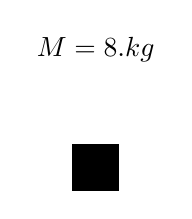
\begin{tikzpicture}[scale=.6]
        \node at (.5,3) {$M=\SI{8.}{kg}$};
        \fill(0,0) rectangle(1,1);
      \end{tikzpicture}
      \hspace{2in}
      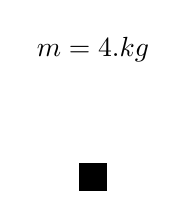
\begin{tikzpicture}[scale=.6]
        \node at (.3,3) {$m=\SI{4.}{kg}$};
        \fill(0,0) rectangle(.6,.6);
      \end{tikzpicture}
    \end{center}

    \vspace{.5in}
    
    \part Calculate the tension in the spring.
    \part Calculate the force constant of the spring.

    \uplevel{
      The string is now cut at point $P$.
    }
    \part Calculate the time taken by the 4.0 kg block to hit the floor
    \part Calculate the frequency of the oscillation of the 8.0 kg block.
    \part Calculate the maximum speed attained by the 8.0 kg block.
  \end{parts}
  \newpage

  \question A 2.0 kg block sits on a 4.0 kg block that is resting on a
  frictionless table, as shown below. The coefficient of friction between the
  blocks are $\mu_s=0.30$ and $\mu_k=0.20$.
  \begin{center}
    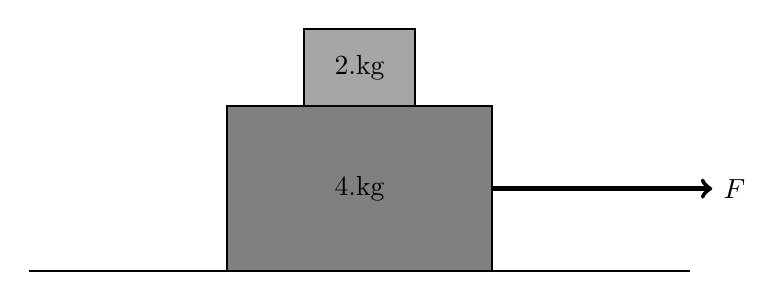
\begin{tikzpicture}[scale=1.4]
      \draw[thick] (0,0)--(6,0);
      \draw[thick,fill=gray] (1.8,0)rectangle(4.2,1.5)
      node[midway,black]{\SI{4.}{kg}};
      \draw[thick,fill=gray!70](2.5,1.5)rectangle(3.5,2.2)
      node[midway]{\SI{2.}{kg}};
      \draw[ultra thick,->](4.2,.75)--(6.2,.75) node[right]{$\bm{F}$};
    \end{tikzpicture}
  \end{center}
  \begin{parts}
    \part What is the maximum force $\bm{F}$ that can be applied if the
    2.0 kg block is not to slide on the 4.0 kg block.
    
    \part If $\bm{F}$ is half this value, find the acceleration of each block
    and the force of friction acting on each block.
    
    \part If $\bm{F}$ is twice the value found in (a), find the acceleration of
    each block.
  \end{parts}
  \newpage
  
  \question A \SI{2.}{\kilo\gram} body rests on a smooth wedge that has an
  inclination of \ang{60} and an acceleration $\bm{a}$ to the right such that
  the mass remains stationary relative to the wedge.
  \begin{center}
    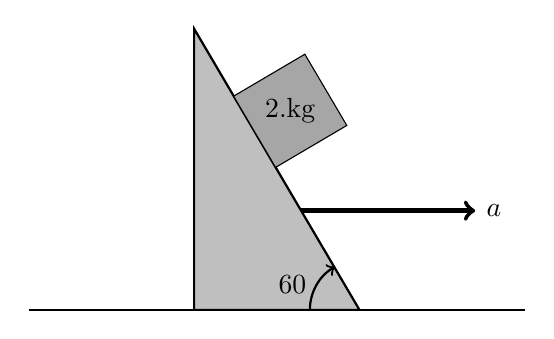
\begin{tikzpicture}[scale=2.1]
      \draw[ultra thick,->](.5,.6)--(1.7,.6) node[right,black]{$\bm{a}$};
      \draw[thick](-1,0)--(2,0);
      \draw[thick,fill=gray!50](0,0)--(0,1.7)--(1,0)--cycle;
      \draw[thick,->](.7,0) arc(180:120:.3) node[midway,left]{\ang{60}};
      \begin{scope}[rotate around={-59.5:(1,0)}]
        \draw[fill=gray!70](0,0) rectangle(-.5,.5)
        node[midway,black]{\SI{2.}{kg}};
      \end{scope}
    \end{tikzpicture}
  \end{center}
  \begin{parts}
    \part Find acceleration $\bm{a}$.
    \part What would happen if the wedge were given a greater acceleration?
  \end{parts}
  \newpage
  
  \question A pick-up truck with two stacked crates in the truck bed brakes
  quickly. The crate on the bottom just barely stays put on the bed of the
  truck. Does the top crate stay put or does it fall off? The top crate has a
  mass of \SI{27}{\kilo\gram} and the mass of the bottom crate is
  \SI{22}{\kilo\gram}. The coefficient of static friction between the bottom
  crate and the truck is 0.42, and the coefficient of kinetic friction for that
  surface is 0.35. The coefficient of static friction between the crate is
  0.40, and the coefficient of kinetic friction is 0.32.
  \newpage
  
%\item  Two blocks of mass $m$ and $M$ are connected via pulley with a
%  configuration as shown on the right. The coefficient of static friction
%  between the left block and the surface is $\mu_{s,1}$, and the coefficient of
%  static friction between the right block and the surface is $\mu_{s,2}$.
%  Formulate a mathematical inequality for the condition that no sliding occurs.
%  There may be more than one inequality.
%  \begin{center}
%    \pic{.4}{pulley_prob_6.png}
%  \end{center}
\end{questions}
\end{document}
